\section{住宿条件}

\subsection*{沙河宿舍简介}

根据宿舍楼的位置,沙河校区的宿舍分为雁北园和雁南园。相对而言,雁北园的条件会差一些,比如阳台空间较小、公共浴室较为破旧和储物空间较少。但其实也只是差一点~

\emph{雁北园}位于鸿雁路北侧,A/B/C/D1是四栋矩形相连的宿舍楼(一楼入口独立,二楼以上的部分相连),D2/E是另两栋独立于A/B/C/D1宿舍楼且相对较小的宿舍楼,内部也是相连的。目前2020级软件工程的学长们就住在这里(等你们入学就要搬去本部了),离食堂操场生活区较近。雁北园各区域的代号为A/B/C/D1/D2/E。

\emph{雁南园}位于鸿雁路南侧,S2 S3 S4 S5是四栋平行的宿舍楼,六层,是2021级学生的主要宿舍楼,离教学楼和学校景观湖(线程池?)较近,南区食堂也修好了,即将投入使用。S6是一栋单独的宿舍楼,由于2020年才投入使用,所以条件是全校最好的。雁南园各区域的代号为S2/S3/S4/S5/S6(S1是信息中心楼)。

学校有三栋教学用楼宇的名字也是S1(教学楼)、S2(学院楼)和S3(实验楼),不要和宿舍楼弄混哦。S2 S3 S4 为男生宿舍,互通;S5 S6为女生宿舍(实际有三个不相通的部分)。按照学校的安排,所有的女生应该会统一入住S5和S6,其余宿舍均为男生宿舍。

\subsection*{宿舍环境}

无论是雁北园还是雁南园,宿舍的基本配置都是:四人间,上床下桌,有独立卫生间。卫生间内只有一个坑位和洗脸面盆,不能洗澡(但有地漏)。有的宿舍楼的独立卫生间会分成两个部分,分别是坑位和洗脸池。厕所里没有垃圾桶,需要自己购买。房间内有空调和暖气片,有阳台。

\begin{center}
    \begin{minipage}{0.45\textwidth}
        \centerline{\fangsong\small 雁北和除S6以外的雁南宿舍}
        \centerline{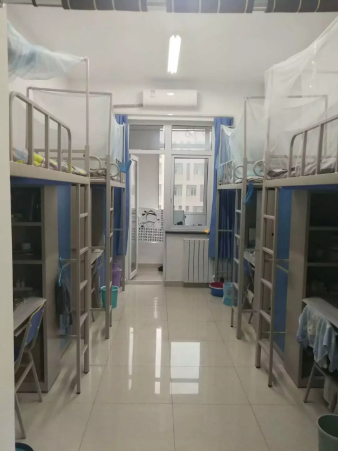
\includegraphics[width=1\textwidth]{images/dorm.png}}
    \end{minipage}
    \qquad
    \begin{minipage}{0.45\textwidth}
        \centerline{\fangsong\small 雁南S6宿舍}
        \centerline{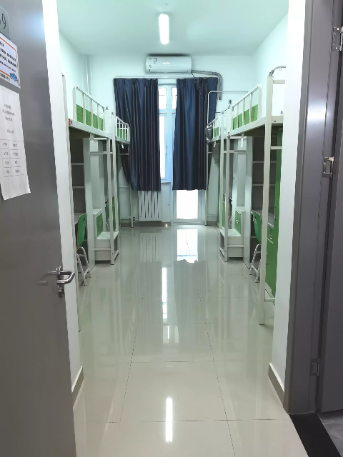
\includegraphics[width=1\textwidth]{images/dorm-s6.png}}
    \end{minipage}
\end{center}

\faq{我需要带什么生活用品吗?}

其实你可以什么也不带,报道当天都可以去学校超市购买。当然你自己带好常用的洗漱用品、床单被套啥的也可以。(建议非必须物品提前物流、网购或现场买,不建议千里迢迢携带)

\faq{宿舍楼还有其他配置吗?}

每层楼有一个公共卫生间和澡堂,(如果不想经常清理房间里的厕所,建议多去公共卫生间),一楼有宿管的值班室,可以使用微波炉。每栋楼有一个电梯,一楼有若干自动售货机(买饮料零食泡面啥的),支持移动支付。部分楼层会有空出的房间作为自习室。

\faq{我会和我的同班同学住一个寝室吗?}

一般会,但也可能和同专业的其他班同学住一起。极端情况下你会与其他专业的同学一个寝室。分寝室结果在报道前可以在信息门户网上查到。

\faq{宿舍楼有门禁吗?}

有,同一栋楼仅允许该楼学生刷卡进入,实际没有,但有宵禁。宿舍楼开放时间是早上6点到晚上11:00,如果要十一点以后回宿舍,就要提前联系辅导员进楼。带外来人员进楼要在宿管处登记。

\faq{澡堂是怎么样的?}

纯淋浴房。采用刷卡计费的方式,大概每分钟0.1元。澡堂中午12:00到晚上23:00开放(其实管的不严的情况下一般不锁门,但最好还是提前去洗),但一般下午四五点以后才有热水。实测全天有热水,多放一会儿即可。

\faq{水电费怎么算?}

水费目前没有收。电费每人每学期赠送40度电。(所以宿舍四个人一共赠送160度)电费价格:12元可购买25度电。(只有空调最花钱,要不然花不了多少电)

\faq{宿舍装饰有什么限制吗,可以拉床帘吗?}

规定上不允许安装床帘,实际执行上不严。有部分宿管会限制蚊帐、床帘和地垫,可以尝试和他们理论,无果的话就不要装啦,具体购买之前可以先询问宿管和辅导员。不可以使用大功率电器(具体到时看宿舍须知)

\faq{上床下桌的尺寸是多大?}

\begin{center}
    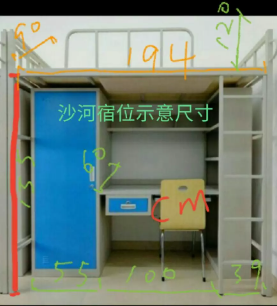
\includegraphics[width=0.55\textwidth]{images/bed-size.png}
\end{center}

又到了搬出老图的时候——不同宿舍的柜子尺寸可能不同,上床离天花板大概一米多一点,桌子上可以放得下27"显示屏。

\faq{辅导员会检查宿舍吗?}

辅导员开学后会有宿舍评比,主要看装饰和整洁度,可能会影响德育分(关于德育分的问题见下),具体看学院政策。辅导员查寝的频率取决于你的导员有多懒,以及学院有没有发动什么相关运动。
每周会有宿管卫生检查(实际上没来过几次),按百分制进行计分,基准分为100不符合规定的倒扣对应分数。
